% Chapter Template

\chapter{Selection of Compatible Polymer-Solvent Combinations for Near-Field Electrospinning and Pyrolysis} % Main chapter title

\label{Chapter:3}

% search : electrospunable capacity vs. thermo analysis of polymers in solutions (bad/good solvents)

Zhenan Bao et al. \cite{Liu2015a} investigated the effect of the polymer chemical structure (the effect of benzene rings) on the morphology, dimensions, composition, graphitization degree, crystallinity, and electrical conductivity of graphene nano-ribbons derived from four different types of electrospun polymers. The authors studied four polymers polystyrene (PS), poly(vinyl alcohol) (PVA), polyvinylphenol (PVP), and a phenolic resin known as Novolac. See Figure \ref{fig:zhenanBaoPolymers}. The authors created  electrospun polymer fibers out of the four selected polymers. PVP, Novolac and PVA have hydroxyl groups that can be functionalized with metal cations, while PS does not have such binding capability. On the other hand, PVP and Novolac have one benzene ring in each repeating unit, wheras PVA is mainly made out of sp3 carbon.

\begin{figure}[!th]
\centering
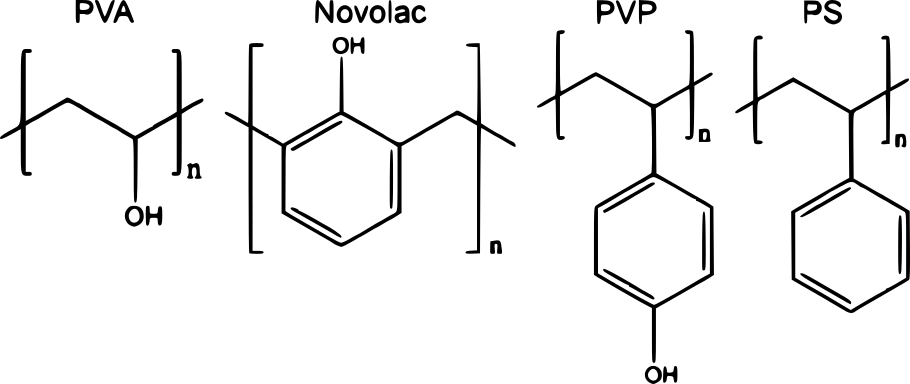
\includegraphics[scale=0.35]{./Figures/zhenanBaoPolymers.png}
\decoRule
\caption[Studied Polymers by Zhenan Bao et al. \cite{Liu2015a}]{Studied Polymers by Zhenan Bao et al. \cite{Liu2015a}}
\label{fig:zhenanBaoPolymers}
\end{figure}

Zhenan Bao et al. \cite{Liu2015a} found that higher sp2 carbon content (or more benzene rings) in the polymer chemical structure translates into higher graphitization degree and higher electrical conductivity in the final carbon structures. This finding can be use as a guide when choosing polymer precursors for the fabrication of carbon structures. Furthermore, the authors posit that polymers with functional groups are required for the creation of smooth and continuous fibers throw electrospinning. \cite{Liu2015a}

%----------------------------------------------------------------------------------------
%	SECTION 1
%----------------------------------------------------------------------------------------
\section{Selection of Candidate Spunable Polymer Solutions}
%high molecular weight, polymer-solution interaction (straight chains)
Given the conclusions from Zhenan Bao et al. \cite{Liu2015a} along with the extensive literature review and data analysis of Chapter \ref{Chapter:2}, the following polymer solutions were selected to be studied in this work. Polymer selection was based on the their high carbon content and presence of benzene rings. The purpose of the polymer selection is to focus the efforts to maximize the likelihood of polymers to yield carbon structures with high electrical conductivity and high graphitization degree; as testing every possible polymer-solvent system is not a practical way to carry on this research. Figure \ref{fig:selectedpolymers} lists the polymers that are going to be investigated. The selected polymers have been electrospun via far-field electrospinning for the fabrication of fibrous mats \cite{Fong1999, Min2013, Yousefi2019}, but no records of being spunable by NFES. 

% PSB 
% PS  192 000
% PSMS
% PVK 1 100 000
% PEO 4 000 000

\begin{figure}[!th]
\centering
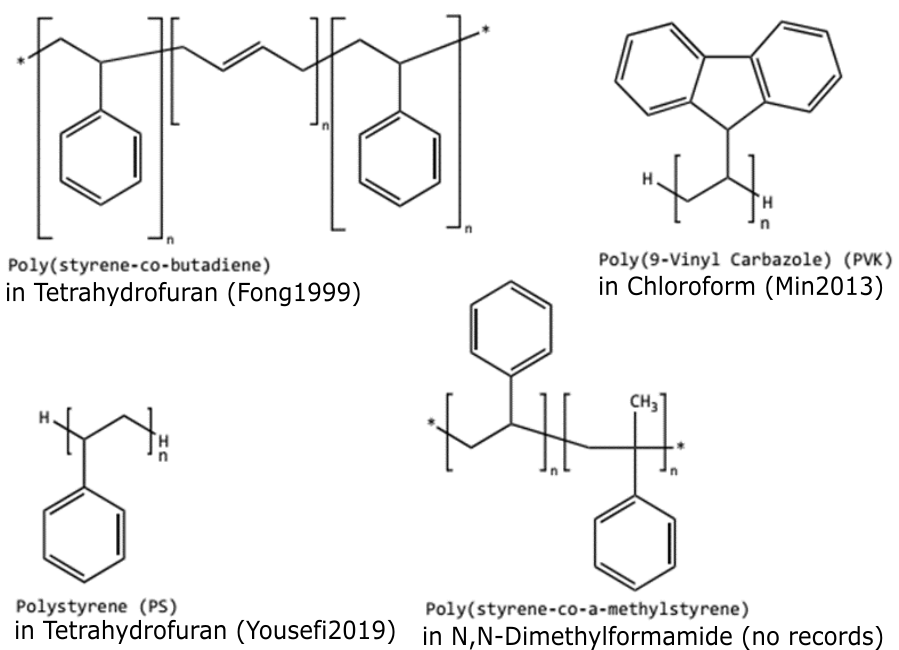
\includegraphics[scale=0.55]{./Figures/selectedpolymers.png}
\decoRule
\caption[Selection of Polymer-Solvent Systems to Investigate in this Work]{Selection of Polymer-Solvent Systems to Investigate in this Work. \cite{Fong1999, Min2013, Yousefi2019}}
\label{fig:selectedpolymers}
\end{figure}

\section{Rheology of candidate polymer solutions}
As stated in previous sections, near-field electrospinning requires the control of several parameters to obtain fibers with the desired properties. One of the main parameters are related to the polymer precursor such as molecular weight and its concentration in solution. The evaluation of polymer chain entanglements is an effective way to address the spunability of a polymer-solvent system. \cite{Shenoy2005} Polymer concentration and molecular weight are the main factors in determining the entanglement degree between polymer chains. 

\begin{figure}[!th]
\centering
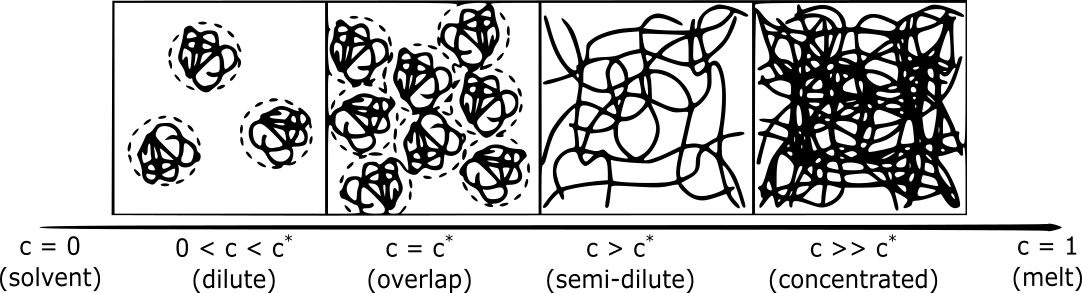
\includegraphics[scale=0.50]{./Figures/criticalConcentrationEntanglement.png}
\decoRule
\caption[Polymer Chain Entanglement in Function of Polymer Concentration]{Effect of the polymer concentration on the structure of polymer chains in solution. Adapted from \cite{Burghelea2020}}
\label{fig:criticalConcentrationEntanglement}
\end{figure}

Solutions at low concentrations do not allow polymer chains to entangle leading the viscoeslasticity od the solution dependent only on individual polymer chains. As the polymer concentration increases, the chains overlap and become entangled. The concentration at which the entanglement initially takes place is the critical concentration $c^*$. Concentrations above the critical concentration $c^*$ generate a fast increase in chain entanglement (Figure \ref{fig:criticalConcentrationEntanglement}). This rapid change in chain entanglement is translated into a fast increase in the viscoelasticity of the solution. Figure \ref{fig:concentrationViscosityPlotExplained} illustrates the relationship between polymer concentration and viscoelasticity. \cite{Burghelea2020, Gupta2005}

\begin{figure}[!th]
\centering
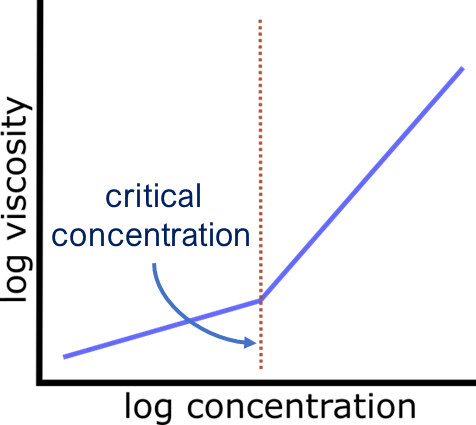
\includegraphics[scale=0.45]{./Figures/concentrationViscosityPlotExplained.png}
\decoRule
\caption[Effect on Solution Viscosity and Related Electrospinning Capability]{Effect on solution viscosity, polymer concentration and spinnability. Adapted from \cite{Burghelea2020, Gupta2005, Han2019}}
\label{fig:concentrationViscosityPlotExplained}
\end{figure}

Electrospinning of smooth, continuous fibers require a polymer concentration higher than the critical concentration. As shown in Figure \ref{fig:concentrationViscosityPlotExplained}, the critical concentration can be estimated from the change in slope. \cite{Burghelea2020, Gupta2005, Han2019} Therefore, in order to find the critical/spinnable concentrations of the candidate polymer-solvent solutions (poly(styrene-co-butadiene) in tetrahydrofuran, poly(9-vinyl carbazole) in chloroform, polyestyrene in tetrahydrofuran, and poly(styrene-co-a-methylstyrene) - See Figure \ref{fig:selectedpolymers}), it is necessary to build the appropriate viscosity vs. concentration plots as described in the following sections.

%\begin{table}[!th]
%\centering
%\caption[Set of Polymer-Solvent Systems to be Analyzed]{Set of Polymer-Solvent Systems to be Analyzed}
%\begin{tabularx}{\textwidth}{ l >{\raggedright\arraybackslash}X }
%\hline
%\textbf{Polymer}                                & \textbf{Solvent}                                      \\
%\hline
%Poly(Ethylene Oxide) (PEO) + SU-8 2002 (SU-8)   & Cyclopentanone                                        \\
%Polystyrene (PS)                                & Tetrahydrofuran (THF)                                 \\
%Poly(Styrene-co-Butadiene) (PSB)                & 1-Methyl-2-Pyrrolidinone (NMP)                        \\
%Poly(Styrene-co-Butadiene) (PSB)                & Tetrahydrofuran (THF) and N,N-Dimethylformamide (DMF) \\
%Poly(Styrene-co-alpha-Methylstyrene) (PSMS)     & N,N-Dimethylformamide (DMF)                           \\
%Poly(9-Vinylcarbazole) (PVK)                    & Chloroform (CHL)                                      \\
%Poly(9-Vinylcarbazole) (PVK) + SU-8 2002 (SU-8) & Cyclopentanone (CPO)                                  \\
%\hline
%\end{tabularx}
%\label{tab:candidatePolymerSolventSystems}
%\end{table}

\subsection{Materials and Sample Preparation}

Seven polymer-solvent combinations are to be tested. The Poly(Ethylene Oxide) and SU-8 2002 combination is what has been used in past work \cite{Cardenas2017, Flores2017}, and will be used as the control sample set. The selected polymer-solvent combinations are to investigate the ability of oxygenless polymers to be electrospun and then carbonized into vitreous carbon. Tables \ref{tab:PEOinSU8}, \ref{tab:PSBinNMP}, \ref{tab:PSBinTHFnDMF}, \ref{tab:PSMSinDMF}, \ref{tab:PSinTHF}, \ref{tab:PVKinCHL}, and \ref{tab:PVKinSU8} list the prepared polymer systems. Tetrabutylammonium tetrafluoroborate (TBF) was added to all solutions to increase the conductivity of the solution. SU-8 contains $71\%$ of cyclopentanone (CPO), which acts as the solvent (Figure \ref{fig:su8Components}) \cite{Microchem2012}.

\begin{table}[!th]
\centering
\caption[Poly(Ethylene Oxide) and SU-8 2002 : Control Sample Preparation]{Poly(Ethylene Oxide) and SU-8 2002 : Sample Preparation}
\begin{tabular}{cccc}
\hline
\textbf{Sample} & \multicolumn{3}{c}{\textbf{Weight Percent} $wt\%$} \\
\hline
{}          & \textbf{SU-8} & \textbf{PEO} & \textbf{TBF} \\
\textbf{ 1} & 99.50         & 0.00         & 0.50         \\
\textbf{ 2} & 99.25         & 0.25         & 0.50         \\
\textbf{ 3} & 99.00         & 0.50         & 0.50         \\
\textbf{ 4} & 98.75         & 0.75         & 0.50         \\
\textbf{ 5} & 98.50         & 1.00         & 0.50         \\
\hline
density $[\textrm{g} / \textrm{ml}]$
   & 1.123         & {}           & {}           \\
\hline
\end{tabular}
\label{tab:PEOinSU8}
\end{table}

\begin{table}[!th]
\centering
\caption[Polystyrene in Tetrahydrofuran : Sample Preparation]{Polystyrene in Tetrahydrofuran : Sample Preparation}
\begin{tabular}{cccc}
\hline
\textbf{Sample} & \multicolumn{3}{c}{\textbf{Weight Percent} $wt\%$} \\
\hline
{}          & \textbf{THF} & \textbf{PS} & \textbf{TBF} \\
\textbf{ 6} & 99.25        &  0.25       & 0.50         \\
\textbf{ 7} & 94.50        &  5.00       & 0.50         \\
\textbf{ 8} & 89.50        & 10.00       & 0.50         \\
\textbf{ 9} & 84.50        & 15.00       & 0.50         \\
\textbf{10} & 79.50        & 20.00       & 0.50         \\
\textbf{11} & 69.50        & 30.00       & 0.50         \\
\textbf{12} & 64.50        & 35.00       & 0.50         \\
\textbf{13} & 59.50        & 40.00       & 0.50         \\
\hline
density $[\textrm{g} / \textrm{ml}]$
   & 0.888        & {}          & {}           \\
\hline
\end{tabular}
\label{tab:PSinTHF}
\end{table}

\begin{table}[!th]
\centering
\caption[Poly(Styrene-co-Butadiene) in 1-Methyl-2-Pyrrolidinone : Sample Preparation]{Poly(Styrene-co-Butadiene) in 1-Methyl-2-Pyrrolidinone : Sample Preparation}
\begin{tabular}{cccc}
\hline
\textbf{Sample} & \multicolumn{3}{c}{\textbf{Weight Percent} $wt\%$} \\
\hline
{}          & \textbf{NMP} & \textbf{PSB} & \textbf{TBF} \\
\textbf{14} & 98.50        &  1.00        & 0.50         \\
\textbf{15} & 95.50        &  4.00        & 0.50         \\
\textbf{16} & 91.50        &  8.00        & 0.50         \\
\textbf{17} & 87.50        & 12.00        & 0.50         \\
\hline
density $[\textrm{g} / \textrm{ml}]$
   & 1.027        & {}           & {}           \\
\hline
\end{tabular}
\label{tab:PSBinNMP}
\end{table}

\begin{table}[!th]
\centering
\caption[Poly(Styrene-co-Butadiene) in Tetrahydrofuran and N,N-Dimethylformamide : Sample Preparation]{Poly(Styrene-co-Butadiene) in Tetrahydrofuran and N,N-Dimethylformamide : Sample Preparation}
\begin{tabular}{ccccc}
\hline
\textbf{Sample} & \multicolumn{4}{c}{\textbf{Weight Percent} $wt\%$} \\
\hline
{}          & \textbf{THF} & \textbf{DMF} & \textbf{PSB} & \textbf{TBF} \\
\textbf{18} & 70.875       & 23.625       &  5.00        & 0.50         \\
\textbf{19} & 69.000       & 23.000       &  7.50        & 0.50         \\
\textbf{20} & 67.125       & 22.375       & 10.00        & 0.50         \\
\textbf{21} & 65.250       & 21.750       & 12.50        & 0.50         \\
\textbf{22} & 63.375       & 21.125       & 15.00        & 0.50         \\
\textbf{23} & 59.625       & 19.875       & 20.00        & 0.50         \\
\textbf{24} & 55.875       & 18.625       & 25.00        & 0.50         \\
\hline
density $[\textrm{g} / \textrm{ml}]$
   & 0.888        & 0.950        & {}           & {}           \\
\hline
\end{tabular}
\label{tab:PSBinTHFnDMF}
\end{table}

\begin{table}[!th]
\centering
\caption[Poly(Styrene-co-alpha-Methylstyrene) in N,N-Dimethylformamide : Sample Preparation]{Poly(Styrene-co-alpha-Methylstyrene) in N,N-Dimethylformamide : Sample Preparation}
\begin{tabular}{cccc}
\hline
\textbf{Sample} & \multicolumn{3}{c}{\textbf{Weight Percent} $wt\%$} \\
\hline
{}          & \textbf{DMF} & \textbf{PSMS} & \textbf{TBF} \\
\textbf{25} & 99.00        &  0.50         & 0.50         \\
\textbf{26} & 94.50        &  5.00         & 0.50         \\
\textbf{27} & 89.50        & 10.00         & 0.50         \\
\textbf{28} & 84.50        & 15.00         & 0.50         \\
\hline
density $[\textrm{g} / \textrm{ml}]$
   & 0.950        & {}           & {}           \\
\hline
\end{tabular}
\label{tab:PSMSinDMF}
\end{table}

\begin{table}[!th]
\centering
\caption[Poly(9-Vinylcarbazole) in Chloroform : Sample Preparation]{Poly(9-Vinylcarbazole) in Chloroform : Sample Preparation}
\begin{tabular}{cccc}
\hline
\textbf{Sample} & \multicolumn{3}{c}{\textbf{Weight Percent} $wt\%$} \\
\hline
{}          & \textbf{CHL} & \textbf{PVK} & \textbf{TBF} \\
\textbf{29} & 99.50        &  0.00        & 0.50         \\
\textbf{30} & 99.49        &  0.01        & 0.50         \\
\textbf{31} & 84.50        & 15.00        & 0.50         \\
\textbf{32} & 79.50        & 20.00        & 0.50         \\
\textbf{33} & 69.50        & 30.00        & 0.50         \\
\hline
density $[\textrm{g} / \textrm{ml}]$
            & 1.492        & {}           & {}           \\
\hline
\end{tabular}
\label{tab:PVKinCHL}
\end{table}

\begin{table}[!th]
\centering
\caption[Poly(9-Vinylcarbazole) and SU-8 2002 : Sample Preparation]{Poly(9-Vinylcarbazole) and SU-8 2002 : Sample Preparation}
\begin{tabular}{cccc}
\hline
\textbf{Sample} & \multicolumn{3}{c}{\textbf{Weight Percent} $wt\%$} \\
\hline
{}          & \textbf{SU-8} & \textbf{PVK} & \textbf{TBF} \\
\textbf{34} & 99.50         &  0.00        & 0.50         \\
\textbf{35} & 99.495        &  0.005       & 0.50         \\
\textbf{36} & 98.75         &  0.75        & 0.50         \\
\textbf{37} & 94.50         &  5.00        & 0.50         \\
\textbf{38} & 79.50         & 20.00        & 0.50         \\
\hline
density $[\textrm{g} / \textrm{ml}]$
   & 1.123         & {}           & {}           \\
\hline
\end{tabular}
\label{tab:PVKinSU8}
\end{table}

\FloatBarrier % keep tables together

SU-8 2002 was obtained from MicroChem (Newton, MA, USA), while Tetrabutylammonium Tetrafluoroborate (TBF) of $99\%$ purity were, Poly(Ethylene Oxide) (PEO), Polystyrene (PS), Poly(Styrene-co-Butadiene) (PSB), Poly(Styrene-co-alpha-Methylstyrene) (PSMS), Poly(9-Vinylcarbazole) (PVK), Tetrahydrofuran (THF), 1-Methyl-2-Pyrrolidinone (NMP), N,N-Dimethylformamide (DMF), and Chloroform (CHL) were obtained from Sigma-Aldrich (Saint Louis, MI, USA). PEO has a viscosity-average molecular weight Mv of ~4,000,000, with less than 1000 ppm of Butylated Hydroxytoluene (BHT) as an inhibitor. PS has an average molecular weight Mw of ~192,000. PSB has a melt index of $6 \textrm{g} / 10 \textrm{min} (200^{\circ}C / 5 \textrm{kg})$, where the butadiene comprises 4 $wt\%$ PSMS has a melt viscosity of $10 \textrm{Pa} \cdot \textrm{s}$ at $161^{\circ}C$. PVK has an average molecular weight Mw of ~1,100,000 in powder form. THF is anhydrous and contained no inhibitor with $99.9\%$ purity. NMP is anhydrous with $99.5\%$ purity. DMF is anhydrous with $99.8\%$ purity. CHL has $99.5\%$ purity, a melting point of $-63^{\circ}C$, boiling point of $60.5^{\circ}C$, and a density of $1.492 \textrm{g} / \textrm{ml}$ at $25^{\circ}C$. CHL contains between 100 to 200 ppm amylenes as stabilizer. SU-8 is a high contrast, epoxy-based negative photoresist. All of the reactants were used as received.

Samples of 3 militers were prepared with the adecuate amounts of polymer, salt and solvent. Solutions were stired at $160 rpm$ for $2 hours$ at $60^{\circ}C$. Samples with higher polymer concentrations often required more stirring time to eliminate all polymer aggregates. All solutions were left undisturbed for $3 hours$ in 4 ml vials to eliminate bubbles from the solution.

\subsection{Rheological Characterization of polymer Solutions}
All of the rheological tests were performed in a rotational rheometer (Discovery Hybrid Rheometer DHR, TA Instruments) equipped with a cone-and-plate (CP) geometry (diameter of $60 mm$, angle of $0.9969^{\circ}$, and truncation of $23 \mu m$) in a steel Peltier plate (Figure \ref{fig:solventTrap}a). The experiments were conducted at $20^{\circ}C$ and $3 hours$ after polymer solution preparation. Flow curve (FC) tests were conducted to obtain viscosity curves in function of the shear rate. Analysis were performed at shear rate range from $10^{-3} \textrm{ 1} / \textrm{s}$ to $10^{4} \textrm{ 1} / \textrm{s}$. A solvent trap cover (Figure \ref{fig:solventTrap}f) and solvent trap geometry (Figure \ref{fig:solventTrap}a) were used to create a thermally stable vapor barrier, virtually eliminating any solvent loss during the rheological experiments and improving temperature uniformity. Distilled water was used to create a seal between the CP geometry and the solvent trap cover (Figure \ref{fig:solventTrap}e).

\begin{figure}[!th]
\centering
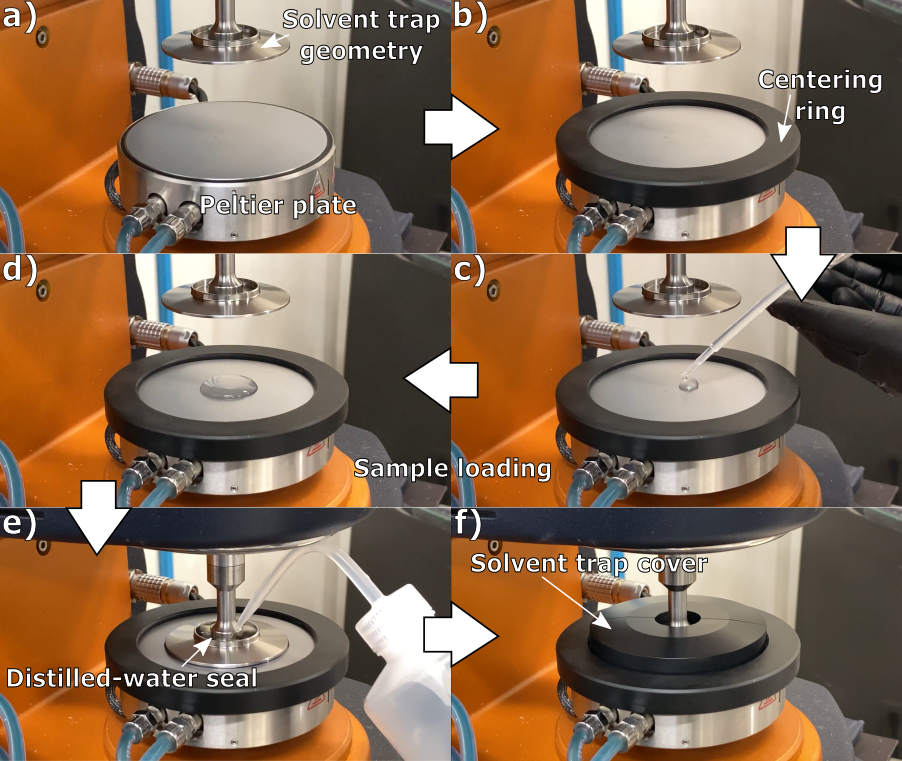
\includegraphics[scale=0.50]{./Figures/solventTrap.png}
\decoRule
\caption[Rheometer - Solvent Trap Setup]{Rheometer - Solvent Trap Setup}
\label{fig:solventTrap}
\end{figure}

Flow curves determine the flow behaviour of a sample by measuring the viscosity as a function of shear rate. For shear rates under $~10^{-2.25} \textrm{ 1} / \textrm{s}$ the rheometer was unable to take viscosity measurements, on the other hand for shar rates over $~10^{-3.5} \textrm{ 1} / \textrm{s}$ the measurements are discarded. At high shear rates, several factors such as inertial effects, and viscous heating can alter the rheometric measurements \cite{RByron1987, Macosko1994}. As the shear rate increases, the centrifugal stresses become large enough to overcome the surface tension stresses that keep the sample within the gap between the geometry and the plate. High centrifugal stresses result in the sample being thrown out of the measuring area; a phenomenon known as 'radial migration effect' \cite{Connelly1985}. Once the 'radial migration effect' partially ejects the sample, the viscosity measurements are lower than expected due to a drop in torque. \cite{Pipe2008}

As depicted in the rheological results in Figures \ref{fig:plt_PEOwtinSU8}, \ref{fig:plt_PSwtinTHF}, \ref{fig:plt_PSBwtinNMP}, \ref{fig:plt_PSBwtinTHFandDMF}, \ref{fig:plt_PSMSwtinDMF}, \ref{fig:plt_PVKwtinCHL} and \ref{fig:plt_PVKwtinSU8}, the constant-viscosity (Newtonian-like) behavior before the shear thinning onset was captured. In all samples, a noticeable shear-thinning behavior is observed with an increase in viscosity with concentration increments. The shear-thinning behavior can be interpreted as the alignment of polymer chains to the flow in the direction of the applied shear stress. \cite{Floreshernandez2020} The Carreau–Yasuda model (Equation \ref{eqn:carreauYasudaModel}) \cite{RByron1987} was fitted to the cone-and-plate  measurements to compute the zero-shear viscosity of each sample.

\begin{equation}\label{eqn:carreauYasudaModel}
    \eta = \frac{\eta_0 - \eta_{\infty}}{\left[1 + \left(\kappa \dot{\gamma}\right)^a\right]^{\frac{(1 - n)}{a}}} + \eta_{\infty}
\end{equation}

Where: $\eta$ is the viscosity, $\dot{\gamma}$ the shear rate, $\eta_{\infty}$ the  infinite shear rate viscosity, $\eta_0$ the zero shear rate viscosity, $\kappa$ is the time constant, $n$ the Power Law index, $a$ the width of the transition region between the zero shear viscosity and the Power Law region. The model was fitted to the rheologial data to estimate $\eta_0$. Then, $\eta_0$ values are used to create diagrams that describe the effect of polymer concentration on the solution viscosity, as described in Figure \ref{fig:concentrationViscosityPlotExplained}. The critical concentrations are calculated from the change in slope in the zero-shear viscosity to concentration relationship as depicted in Figure \ref{fig:criticalConcentrationCalculation} for the PEO in SU-8 solutions. Appendix \ref{Appendix_CriticalConcentrations} contains the diagrams of the other polymer-solvent systems.

\begin{figure}[!th]
\centering
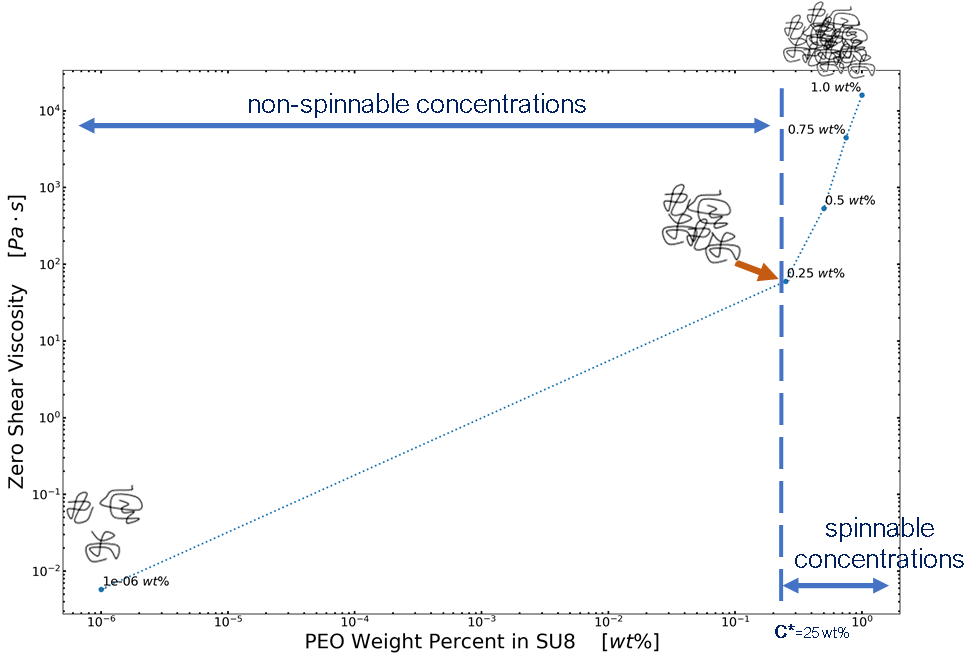
\includegraphics[width=\textwidth]{./Figures/criticalConcentrationCalculation.png}
\decoRule
\caption[Estimation of the Critical Concentration of the PEO in SU-8 solutions]{The change in slope is given at 25 $wt\%$ PEO, which suggests that at 25 $wt\%$ the polymer chains are entangled.}
\label{fig:criticalConcentrationCalculation}
\end{figure}

\begin{table}[!th]
\centering
\caption[Calculated Critical/Spinnable Concentrations for each Polymer-Solvent System]{Calculated Critical/Spinnable Concentrations for each Polymer-Solvent System}
\begin{tabular}{lllll}
\hline
\textbf{Polymer} & \textbf{Molecular Weight $[\textrm{g} \cdot \textrm{mol}]$} & \textbf{Solvent} & \textbf{$c^* [\textrm{wt}\%]$} & \textbf{$\eta_0 [\textrm{Pa} \cdot \textrm{s}]$} \\
\hline
PEO  & 4,000,000                  & CPO (SU-8)  & 0.25  & 60.022 \\
PS   & 192,000                    & THF         & 20.00 & 0.166  \\
PSB  & 490,000   \cite{Doan2013}  & NMP         & 8.00  & 0.028  \\
PSB  & 490,000   \cite{Doan2013}  & THF and DMF & 15.00 & 0.092  \\
PSMS & 2,658,076 \cite{Colby1987} & DMF         & 5.00  & 0.282  \\
PVK  & 1,100,000                  & CHL         & 15.00 & 41.861 \\
PVK  & 1,100,000                  & CPO (SU-8)  & 0.75  & 49.657 \\
\hline
\end{tabular}
\label{tab:calculatedSpinnableConcentrations}
\end{table}

Table \ref{tab:calculatedSpinnableConcentrations} summarizes the calculated critical concentrations for each system. In general, the critical concentration $c^*$ has proportional relationship with the polymer molecular weight, as a polymer's molecular weight greatly influences the solution viscosity. First, the structure of the polymer chain has an effect on its solubility as the intermolecular interactions between long molecules are stronger and the solvent molecules take longer to diffuse within the polymer aggregates. \cite{Ramakrishna2005, Floreshernandez2020} Second, the viscosity of a polymer solution will be smaller when a polymer of low molecular weight is dissolved than a solution of the same polymer but of a higher molecular weight. \cite{Ramakrishna2005} The molecular weight of the polymer describes the length of the polymer chain, which has an effect on the viscosity of the solution. Since the polymer length defines the amount of entanglement of the polymer chains in the solvent, a lower molecular weight shall be compensated by higher concentrations to reach the desired viscosity.